\section{Manejo de Figuras: Tablas, Gráficos e Imágenes}
\LaTeX ofrece potentes herramientas para incluir y formatear figuras, tablas e imágenes con precisión tipográfica. 

\subsection{Manejo de Tablas}
\LaTeX{} ofrece control preciso sobre tablas mediante entornos \texttt{tabular} y \texttt{table} \cite{latex_project}. La principal diferencia entre ambos es que \texttt{tabular} se usa para crear la estructura de la tabla, mientras que \texttt{table} es un entorno flotante que permite agregar títulos, etiquetas y controlar la posición de la tabla en el documento.

\subsubsection{Tabla Básica: Entorno tabular}

En su forma más simple, el entorno \texttt{tabular} se utiliza para crear tablas sin título ni numeración, como se muestra en el siguiente ejemplo:

\begin{tabular}{|l|c|r|}   
\hline 
\textbf{Nombre} & \textbf{Edad} & \textbf{Ciudad} \\
\hline
Juan Pérez & 25 & San José \\
María Gómez & 30 & Alajuela \\
\hline
\end{tabular}

Para crear esta tabla, se utiliza el siguiente código:

\begin{verbatim}
\begin{tabular}{|l|c|r|}
\hline
\textbf{Nombre} & \textbf{Edad} & \textbf{Ciudad} \\
\hline
Juan Pérez & 25 & San José \\
María Gómez & 30 & Alajuela \\
\hline
\end{tabular}
\end{verbatim}

\subsubsection{Tabla Flotante Completa}

Como se mencionó anteriormente, la tabla tabular no permite agregar títulos ni etiquetas para referencias cruzadas. Para esto, se utiliza el entorno \texttt{table}, que es un entorno flotante \cite{latex_project}. Esto significa que LaTeX puede mover la tabla a una posición óptima en el documento, como la parte superior o inferior de una página.

\begin{table}[h]
\centering
\caption{Ejemplo de tabla flotante}
\label{tab:tabla_ejemplo}
\begin{tabular}{lccc}
\toprule
\textbf{Nombre} & \textbf{Edad} & \textbf{Ciudad} \\
\midrule
Juan Pérez & 25 & San José \\
María Gómez & 30 & Alajuela \\
\bottomrule
\end{tabular}
\end{table}

El siguiente código muestra cómo crear una tabla flotante con título y etiqueta, tal como se observa en el Cuadro \ref{tab:tabla_ejemplo}:

\begin{verbatim}
\begin{table}[h] % h=here, t=top, b=bottom
\centering
\caption{Ejemplo de tabla flotante}
\label{tab:tabla_ejemplo}
\begin{tabular}{lccc}
\toprule
\textbf{Nombre} & \textbf{Edad} & \textbf{Ciudad} \\
\midrule
Juan Pérez & 25 & San José \\
María Gómez & 30 & Alajuela \\
\bottomrule
\end{tabular}
\end{table}
\end{verbatim}

\subsection{Manejo de Gráficos e Imágenes}

Para incluir gráficos e imágenes, se utiliza el paquete \texttt{graphicx} \cite{graphicx}. Este paquete permite insertar imágenes en formatos comunes como PNG, JPEG y PDF, y ofrece opciones para escalar, rotar y recortar las imágenes.

\subsubsection{Figuras Individuales}

La siguiente figura muestra un ejemplo de cómo incluir una imagen utilizando el paquete \texttt{graphicx}:

\begin{figure}[h]
\centering
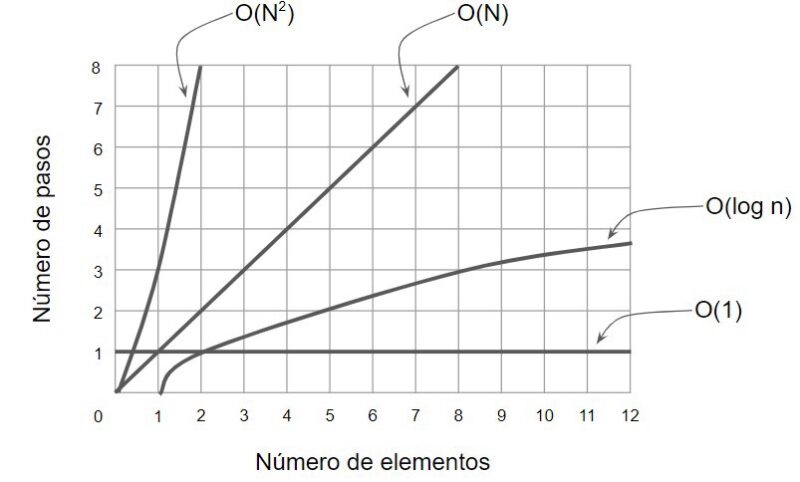
\includegraphics[width=0.45\textwidth]{ejemplo_imagen.jpg}
\caption{Ejemplo de imagen.}
\label{fig:ejemplo_imagen}
\end{figure}

Para insertar la Figura \ref{fig:ejemplo_imagen}, se utiliza el siguiente código:

\begin{verbatim}
\usepackage{graphicx}     % Paquete esencial
\begin{figure}[h]
\centering
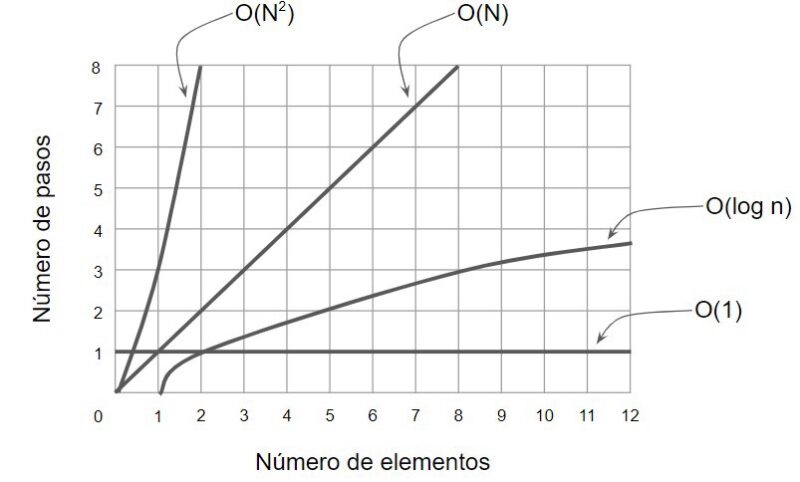
\includegraphics[width=0.45\textwidth]
{ejemplo_imagen.jpg}
\caption{Ejemplo de imagen}
\label{fig:ejemplo_imagen}
\end{figure}
\end{verbatim}

La Figura \ref{fig:ejemplo_imagen} se escaló al 45\% del ancho del texto, pero también se pueden usar otras opciones como \texttt{height} para establecer una altura fija o \texttt{scale} para escalar proporcionalmente:

\begin{verbatim}
\includegraphics[height=5cm]{fig}
\includegraphics[scale=0.5]{fig}
\end{verbatim}

\subsubsection{Subfiguras Múltiples}



\begin{verbatim}
\usepackage{subcaption}
\begin{figure}[h]
\centering
\begin{subfigure}{0.45\textwidth}
\includegraphics[width=\textwidth]{fig1}
\caption{Configuración A}
\label{fig:sub1}
\end{subfigure}
\hfill
\begin{subfigure}{0.45\textwidth}
\includegraphics[width=\textwidth]{fig2}
\caption{Configuración B}
\label{fig:sub2}
\end{subfigure}
\caption{Comparativa experimental}
\label{fig:completa}
\end{figure}
\end{verbatim}

\subsubsection{Gráficos con TikZ (Vectoriales)}

\begin{verbatim}
\usepackage{tikz}
\begin{figure}[h]
\centering
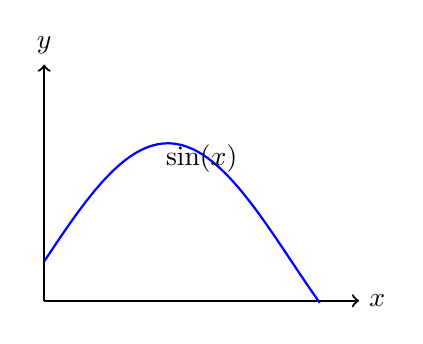
\begin{tikzpicture}
\draw[thick,->] (0,0) -- (4,0) node[right]{$x$};
\draw[thick,->] (0,0) -- (0,3) node[above]{$y$};
\draw[domain=0:3.5,smooth,blue,thick] 
    plot (\x, {sin(\x r)*1.5+0.5});
\node at (2,1.8) {$\sin(x)$};
\end{tikzpicture}
\caption{Función seno generada con TikZ.}
\label{fig:tikz}
\end{figure}
\end{verbatim}

\subsection{Posicionamiento de Flotantes}

\begin{verbatim}

\begin{figure}[htbp!]    % ! fuerza posición
\centering
% Figura aquí
\end{figure}

% Posiciones:
% h = here (aquí)
% t = top (arriba página)
% b = bottom (abajo página) 
% p = page (página flotante)
\end{verbatim}

\subsection{Ejemplo IEEE: Tabla* y Figure* (2 columnas)}

\begin{verbatim}
\begin{table*}
\centering
\caption{Tabla ancha IEEE (abarca 2 columnas)}
% Tabla grande aquí
\end{table*}

\begin{figure*}[t]
\centering
\includegraphics[width=\textwidth]{grafico_grande}
\caption{Figura ancha IEEE}
\end{figure*}
\end{verbatim}
